\documentclass[paper=letter,11pt]{scrartcl}

\KOMAoptions{headinclude=true, footinclude=false}
\KOMAoptions{DIV=14, BCOR=5mm}
\KOMAoptions{numbers=noendperiod}
\KOMAoptions{parskip=half}
\addtokomafont{disposition}{\rmfamily}
\addtokomafont{part}{\LARGE}
\addtokomafont{descriptionlabel}{\rmfamily}
%\setkomafont{pageheadfoot}{\normalsize\sffamily}
\setkomafont{pagehead}{\normalsize\rmfamily}
%\setkomafont{publishers}{\normalsize\rmfamily}
\setkomafont{caption}{\normalfont\small}
\setcapindent{0pt}
\deffootnote[1em]{1em}{1em}{\textsuperscript{\thefootnotemark}\ }


\usepackage{amsmath}
\usepackage[varg]{txfonts}
\usepackage[T1]{fontenc}
\usepackage{graphicx}
\usepackage{xcolor}
\usepackage[american]{babel}
% hyperref is needed in many places, so include it here
\usepackage{hyperref}

\usepackage{xspace}
\usepackage{multirow}
\usepackage{float}


\usepackage{braket}
\usepackage{bbm}
\usepackage{relsize}
\usepackage{tcolorbox}

\def\ketY{\ensuremath{\ket {\Psi}}}
\def\iGeV{\ensuremath{\textrm{GeV}^{-1}}}
%\def\mp{\ensuremath{m_{\textrm{proton}}}}
\def\rp{\ensuremath{r_{\textrm{proton}}}}
\def\me{\ensuremath{m_{\textrm{electron}}}}
\def\aG{\ensuremath{\alpha_G}}
\def\rAtom{\ensuremath{r_{\textrm{atom}}}}
\def\rNucl{\ensuremath{r_{\textrm{nucleus}}}}
\def\GN{\ensuremath{\textrm{G}_\textrm{N}}}
\def\ketX{\ensuremath{\ket{\vec{x}}}}
\def\ve{\ensuremath{\vec{\epsilon}}}


\def\ABCDMatrix{\ensuremath{\begin{pmatrix} A &  B  \\ C  & D \end{pmatrix}}}
\def\xyprime{\ensuremath{\begin{pmatrix} x' \\ y' \end{pmatrix}}}
\def\xyprimeT{\ensuremath{\begin{pmatrix} x' &  y' \end{pmatrix}}}
\def\xy{\ensuremath{\begin{pmatrix} x \\ y \end{pmatrix}}}
\def\xyT{\ensuremath{\begin{pmatrix} x & y \end{pmatrix}}}

\def\IMatrix{\ensuremath{\begin{pmatrix} 0 &  1  \\ -1  & 0 \end{pmatrix}}}
\def\IBoostMatrix{\ensuremath{\begin{pmatrix} 0 &  1  \\ 1  & 0 \end{pmatrix}}}
\def\JThree{\ensuremath{\begin{pmatrix}    0 & -i & 0  \\ i & 0  & 0 \\ 0 & 0 & 0 \end{pmatrix}}} 
\def\JTwo{\ensuremath{\begin{bmatrix}    0 & 0 & -i  \\ 0 & 0  & 0 \\ i & 0 & 0 \end{bmatrix}}}
\def\JOne{\ensuremath{\begin{bmatrix}    0 & 0 & 0  \\ 0 & 0  & -i \\ 0 & i & 0 \end{bmatrix}}}
\def\etamn{\ensuremath{\eta_{\mu\nu}}}
\def\Lmn{\ensuremath{\Lambda^\mu_\nu}}
\def\dmn{\ensuremath{\delta^\mu_\nu}}
\def\wmn{\ensuremath{\omega^\mu_\nu}}
\def\be{\begin{equation*}}
\def\ee{\end{equation*}}
\def\bea{\begin{eqnarray*}}
\def\eea{\end{eqnarray*}}
\def\bi{\begin{itemize}}
\def\ei{\end{itemize}}
\def\fmn{\ensuremath{F_{\mu\nu}}}
\def\fMN{\ensuremath{F^{\mu\nu}}}
\def\bc{\begin{center}}
\def\ec{\end{center}}
\def\nus{$\nu$s}

\def\adagger{\ensuremath{a_{p\sigma}^\dagger}}
\def\lineacross{\noindent\rule{\textwidth}{1pt}}

\newcommand{\multiline}[1] {
\begin{tabular} {|l}
#1
\end{tabular}
}

\newcommand{\multilineNoLine}[1] {
\begin{tabular} {l}
#1
\end{tabular}
}



\newcommand{\lineTwo}[2] {
\begin{tabular} {|l}
#1 \\
#2
\end{tabular}
}

\newcommand{\rmt}[1] {
\textrm{#1}
}


%
% Units
%
\def\m{\ensuremath{\rmt{m}}}
\def\GeV{\ensuremath{\rmt{GeV}}}
\def\pt{\ensuremath{p_\rmt{T}}}


\def\parity{\ensuremath{\mathcal{P}}}

\usepackage{cancel}
\usepackage{ mathrsfs }
\def\bigL{\ensuremath{\mathscr{L}}}

\usepackage{ dsfont }



\usepackage{fancyhdr}
\fancyhf{}


\lhead{\Large 33-444} % \hfill Introduction to Particle Physics \hfill Spring 2019}
\chead{\Large Introduction to Particle Physics} % \hfill Spring 2019}
\rhead{\Large Spring 2020} % \hfill Introduction to Particle Physics \hfill Spring 2019}
\begin{document}
\thispagestyle{fancy}





%\begin{tabular}{c}
%{\large 33-444 \hfill Intro To Particle \hfill Spring 2019\\}
%\hline 
%\end{tabular}

\begin{center}
{\huge \textbf{Midterm 2}}
\large

\end{center}

{\large

\textbf{1) List or draw a diagram of the particles in the Standard model. } \hfill \textit{(6 points)}\\
What is the spin of each particle ?


\underline{Fermions:}, All spin 1/2
\be
\begin{pmatrix} \nu_e \\ e \end{pmatrix} \hspace*{0.1in} \begin{pmatrix} \nu_\mu \\ \mu \end{pmatrix} \hspace*{0.1in}  \begin{pmatrix} \nu_\tau \\ \tau \end{pmatrix}  \hspace*{1in}  \begin{pmatrix} u \\ d \end{pmatrix} \hspace*{0.1in}   \begin{pmatrix} c \\ s \end{pmatrix} \hspace*{0.1in}   \begin{pmatrix} t \\ b \end{pmatrix}  \times \rmt{3 colors}
\ee

\underline{Gauge Bosons:} All spin-1
\be
g \times \rmt{8 colors}  \hspace*{0.2in} W^\pm  \hspace*{0.2in} Z  \hspace*{0.2in} \gamma 
\ee


\underline{Higgs Boson:} spin-0
\be
H
\ee

\vspace*{0.5in}


\textbf{2) Why is the weak interaction so much weaker than then electromagnetic interactions at low energies?} \hfill \textit{(2 points)}\\

\bc
Weak force has massive force carriers.\\
\ec

\clearpage

\textbf{3) Feynman Diagrams }\hfill \textit{(12 points)}\\
Fermions of type $x$ scatter into fermions of type $y$ through the diagram shown below, where $S$ is a massive scalar. 
At low energies ($P_x P_y << m_S$) the cross section for this process is given by $\sigma_0$.
Assume $m_x$ and $m_y$ are both negligible.
\bc
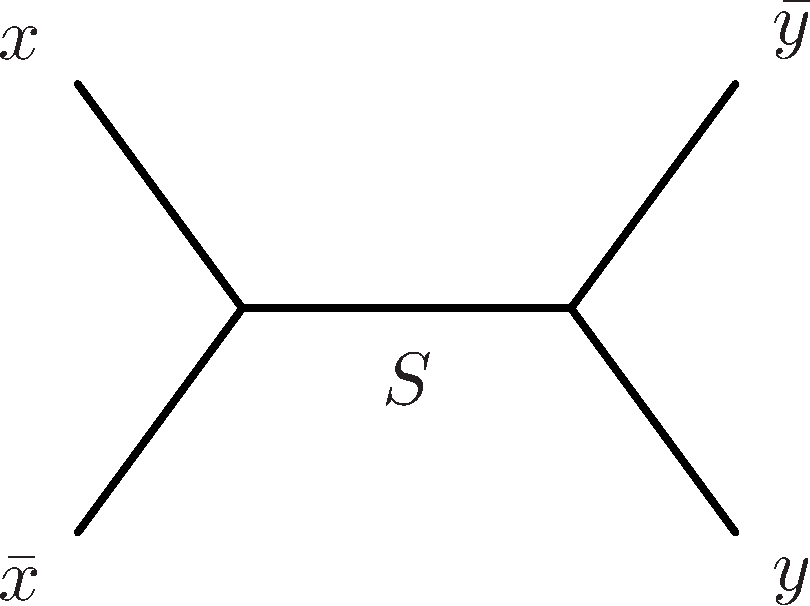
\includegraphics[width=0.2\textwidth]{./xxToyy.pdf}
\ec
\bi
\item[a)] How does this cross section change if the ``S-charge'' of the $x$ particle is doubled ? \\ (S-charge being the $x\bar{x} \rightarrow S$ coupling) 
\be
\sigma \sim |M|^2 \hspace*{0.5in} M \sim q_s
\ee

\be
q_s\rightarrow 2q_s \Rightarrow M \rightarrow 2M \Rightarrow \sigma \rightarrow 4\sigma
\ee
%\vspace*{1.5in}
\item[b)] How does the cross section change if the mass of the $S$-particle is doubled ?
\be
\sigma \sim |M|^2 \hspace*{0.5in} M \sim \frac{1}{M_S^2}
\ee

\be
M_S\rightarrow 2M_S \Rightarrow M \rightarrow \frac{1}{4}M \Rightarrow \sigma \rightarrow \frac{1}{16}\sigma
\ee

\item[c)] At low energies, how does the cross section depend on the center of mass energy of the scattering $E_{CM}$ ? 
\textit{(Hint: At low energies you can think of the $xx \rightarrow yy$ scattering as described by an effective 4-point $xxyy$ interaction, as Fermi did for neutrino scattering.)}

At low energies the scattering is described by an effective 4-point $xxyyy$ interaction.
The xxyy vertex has 4 fermions which each have mass dimension $\frac{3}{2}$.  
So the diagram has mass dimension $[g_{xxyy}] 4 \times \frac{3}{2} = [g_{xxyy}] \times 6$. 
In order to have overall mass dimension four, the mass dimension of the coupling $[g_{xxyy}]$ must be $\GeV^{-2}$.

\be
M \sim \GeV^{-2} \Rightarrow |M|^2 \sim \GeV^{-4}
\ee

Dimensions of $\sigma$ have to work out to be $\GeV^{-2}$.

The only other energy scale in the problem is $E_{CM}$ so.

\be
\sigma \sim \frac{E_{CM}^2}{\GeV^{4}}
\ee

\ei


\textbf{4) Di-boson physics:  } \hfill \textit{(6 points)}\\
Processes in which pairs of gauge bosons are produced are a sensitive probe of the electro-weak theory. These are typically studied at the LHC by looking for signatures involving electrons or muons.  
Estimate how often a $WZ$ event decays into an electron or muon and three neutrinos.\\ ie: $e\nu\nu\nu$ or $\mu\nu\nu\nu$

\bc
$W \rightarrow \ell\nu$ (where $\ell$ is $\mu$ or $e$) is $\frac{2}{3+3\times 2} = \frac{2}{9}$ \\
$Z \rightarrow \nu\nu$  is $\frac{3}{3+3+3\times 5} = \frac{3}{21}$ \\
So, $WZ \rightarrow \ell\nu\nu\nu$ (where $\ell$ is $\mu$ or $e$) is $\frac{2}{9} \times \frac{3}{21} = \frac{2}{63} \sim 3\%$
\ec

\vspace{0.5in}

\textbf{5) Collider Detectors  } \hfill \textit{(4 points)}\\
\begin{itemize}
\item[a)]{ In what ways do the detector signatures of electrons and muons look a-like, in what ways are they different ?

\bi
\item[-]Both have tracks in the inner tracking detector. 
\item[-]Electrons shower in the EM calorimeter and stop, $\mu$s make it through the calorimeter to the muon detector.
\ei

}
\item[b)]{ In what ways do the detector signatures of electrons and photons look a-like, in what ways are they different ?

\bi
\item[-]Both shower in the EM calorimeter and stop.
\item[-]Electrons have a track in the inner tracking detector, photons do not.
\ei


}
\end{itemize}

\vspace*{0.2in}

\textbf{6) Calorimeters } \hfill \textit{(4 points)}\\
Which are more challenging to accurately measure and why : Hadronic showers or electro-magnetic showers? 

Hadronic showers
\bi
\item[-] More complicated:  Multiple lengths scales interaction and radiation lengths important
\item[-] Less particles:  hadrons are heavier so you get less per unit input energy
\item[-] Longer: require more material to contain. 
\ei



\textbf{7) For a new particle X with mass $\sim$ 2 TeV,  would you expect to measure the X mass more precisely from $X\rightarrow ee$ or $X \rightarrow \mu\mu$ ? Justify your answer.} \hfill \textit{(4 points)}\\

X$\rightarrow$ ee
\bi
\item[-] Electrons energies are measured in the calorimeter, which gets more accurate at high energies
\item[-] Muons energies are measured in the trackers (inner and muon), which gets less accurate at high energies
\ei

\vspace*{0.5in}



\textbf{8) How are \nus\ detected at the LHC ?} \hfill \textit{(2 points)}\\

\bc
By looking for momentum imbalance in the transverse plane.
\ec


\textbf{9) The God Particle } \hfill \textit{(4 points)} \\ 
Critique the statement:  ``The Higgs Boson (or god particle) is responsible for all the mass in the Universe''

\bi
\item[-] The Higgs Field is responsible for mass not the Higgs boson
\item[-] The Higgs Boson has nothing to do with God
\item[-] It is responsible for some mass in the univierse (the fundamental particles) not the proton or neutron mass (which are most of the observed (baryonic) mass in the universe) 
\ei

\vspace*{0.3in}



\textbf{10) Higgs Boson Production : } \hfill \textit{(4 points)}\\
Why is Higgs boson production so much rarer then W or Z production despite the fact that their masses are similar?    


\bi
\item[-] It couples very weakly to light particles
\item[-] Production is from higher-order diagrams
\ei


\vspace*{0.3in}


%\textbf{4) Higgs Boson discovery: } \hfill \textit{(5 points)}\\
%The Higgs boson was discovered in its decays to $WW (Br\sim20\%)$, $ZZ\ (Br\sim3\%)$ and $\gamma\gamma\ (Br\sim0.2\%)$.
%However for the $WW$ and $ZZ$ decays, only the ``fully-leptonic'' channels -- where each boson decays leptonicically to $e$ or $\mu$ -- were used. \\
%
%Estimate how often $WW \rightarrow \ell\nu\ell'\nu'$ and $ZZ\rightarrow\ell\ell\ell'\ell'$, where $\ell$ is e or $\mu$. (ignore decays through taus)\\
%
%\bc
%$W \rightarrow \ell\nu$ (where $\ell$ is $\mu$ or $e$) is $\frac{2}{3+3\times 2} = \frac{2}{9}$ \\
%$Z \rightarrow \ell\ell$  (where $\ell$ is $\mu$ or $e$) is $\frac{2}{3+3+3\times 5} = \frac{2}{21}$ \\
%So $WW\rightarrow \ell\nu\ell'\nu' = \frac{2}{9}\times\frac{2}{9} = \frac{4}{81} \sim 5\%$ \\
%And $ZZ\rightarrow \ell\ell\ell'\ell = \frac{2}{21}\times\frac{2}{21} = \frac{4}{441} \sim 1\%$
%\ec
%
%Including these factors, rank the Higgs boson discovery channels by how many signal events they are expected to have.
%
%\bc
%$H\rightarrow WW \rightarrow \ell\nu\ell'\nu' = 0.2(H\rightarrow WW) \times 0.05 (WW\rightarrow\ell\nu\ell'\nu') \sim 1\%$\\
%$H\rightarrow \gamma\gamma = 0.2\% $\\
%$H\rightarrow ZZ\rightarrow\ell\ell\ell'\ell' = 0.03 (H\rightarrow ZZ) \times 0.01 (ZZ\rightarrow\ell\ell\ell'\ell') \sim 0.03\%  $
%\ec
%
%\vspace{0.5in}
%
%\textbf{5) Accelerators: } \hfill \textit{(4 points)}\\
%\begin{itemize}
%\item[a)]{What limits the energy of circular proton accelerators ?
%\bc
%Strength of bending magnets.
%\ec
%}
%\item[b)]{What limits the energy of circular electron accelerators ?
%\bc
%Losses due to Bremstralung radiation loss.
%\ec
%
%}
%\end{itemize}
%
%\clearpage
%
%\textbf{6) Electron-positron Collisions } \hfill \textit{(6 points)}\\
%\begin{itemize}
%\item[a)]{
%How does the value of $R(E_{CM}) \equiv \sigma(ee\rightarrow \rmt{jets})/\sigma(ee\rightarrow \mu\mu)$ change as $E_{CM}$ is increased beyond twice the mass of the charm quark? 
%What values of $R(< 2 m_{\rmt{charm}})$ and $R(> 2 m_{\rmt{charm}})$ do you expect?
%\bc
%Before charm production,  the allowed ``jets'' are  $uu$ (with charge +2/3), dd and ss with charge (-1/3) all have a factor of 3 for color\\
%So $R(< 2 m_{\rmt{charm}}) = 3\times \sum Q^2 = 3 \times \left( (\frac{2}{3})^2 + (\frac{-1}{3})^2  + (\frac{-1}{3})^2  \right) = 3 \times \frac{6}{9} = 2 $ \\
%With charm production,  there is an additional allowed ``jets'' with  $cc$ (with charge +2/3) and a factor of 3 for color\\
%So $R(> 2 m_{\rmt{charm}}) = 3\times \sum Q^2 = 3 \times \left( (\frac{2}{3})^2 + (\frac{-1}{3})^2  + (\frac{-1}{3})^2 + ( \frac{2}{3})^2 \right) = 3 \times \frac{10}{9} \sim 3 $ 
%
%\ec
%}
%
%\item[b)]{Sketch a graph of the total cross section of $ee\rightarrow\mu\mu$ as a function of $E_{CM}$ from 40 GeV to 200. 
%Also sketch the component of the cross section due to the electro-magnetic interaction.
%\bc
%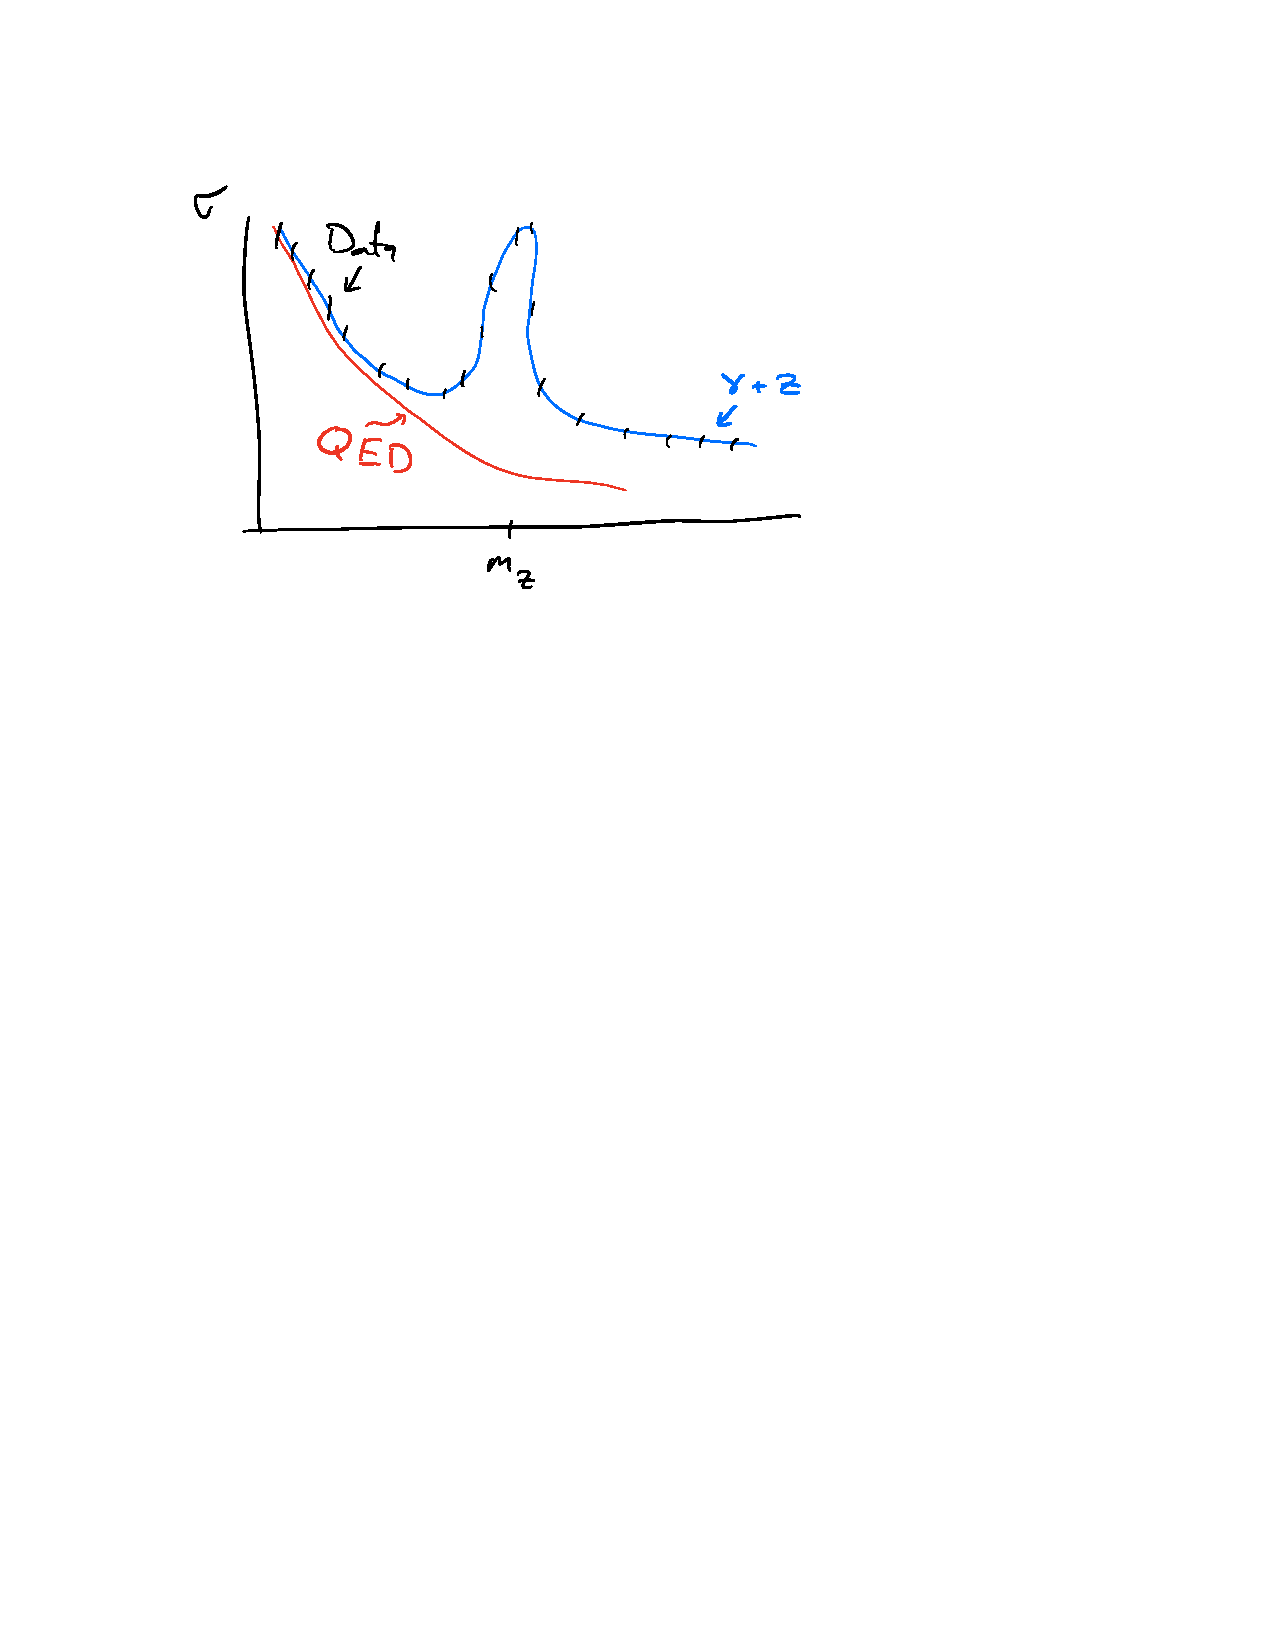
\includegraphics[width=0.4\textwidth]{./ZPeak.pdf}
%\ec
%}
%\end{itemize}

%\vspace*{0.5in}
%
%\textbf{7) Collider Detectors  } \hfill \textit{(4 points)}\\
%\begin{itemize}
%\item[a)]{ In what ways do the detector signatures of electrons and muons look a-like, in what ways are they different ?
%
%\bi
%\item[-]Both have tracks in the inner tracking detector. 
%\item[-]Electrons shower in the EM calorimeter and stop, $\mu$s make it through the calorimeter to the muon detector.
%\ei
%
%}
%\item[b)]{ In what ways do the detector signatures of electrons and photons look a-like, in what ways are they different ?
%
%\bi
%\item[-]Both shower in the EM calorimeter and stop.
%\item[-]Electrons have a track in the inner tracking detector, photons do not.
%\ei
%
%
%}
%\end{itemize}
%
%\vspace*{0.5in}
%        
%
%\textbf{8) Calorimeters } \hfill \textit{(4 points)}\\
%Which are more challenging to accurately measure and why : Hadronic showers or electro-magnetic showers? 
%
%Hadronic showers
%\bi
%\item[-] More complicated:  Multiple lengths scales interaction and radiation lengths important
%\item[-] Less particles:  hadrons are heavier so you get less per unit input energy
%\item[-] Longer: require more material to contain. 
%\ei
%
%\vspace*{0.5in}
%
%
%\textbf{9) For a new particle X with mass $\sim$ 2 TeV,  would you expect to measure the X mass more precisely from $X\rightarrow ee$ or $X \rightarrow \mu\mu$ ? Justify your answer.} \hfill \textit{(3 points)}\\
%
%X$\rightarrow$ ee
%\bi
%\item[-] Electrons energies are measured in the calorimeter, which gets more accurate at high energies
%\item[-] Muons energies are measured in the trackers (inner and muon), which gets less accurate at high energies
%\ei
%
%\vspace*{0.5in}
%
%
%\textbf{10) How are \nus\ detected at the LHC ?} \hfill \textit{(2 points)}\\
%
%\bc
%By looking for momentum imbalance in the transverse plane.
%\ec
%
%\vspace*{0.5in}
%
%\clearpage
%
%\textbf{11) Higgs Boson Production : } \hfill \textit{(4 points)}\\
%\begin{itemize}
%\item[a)]{ Draw one possible Feynman diagram for production and decay of the Higgs boson at the LHC.}
%\bc
%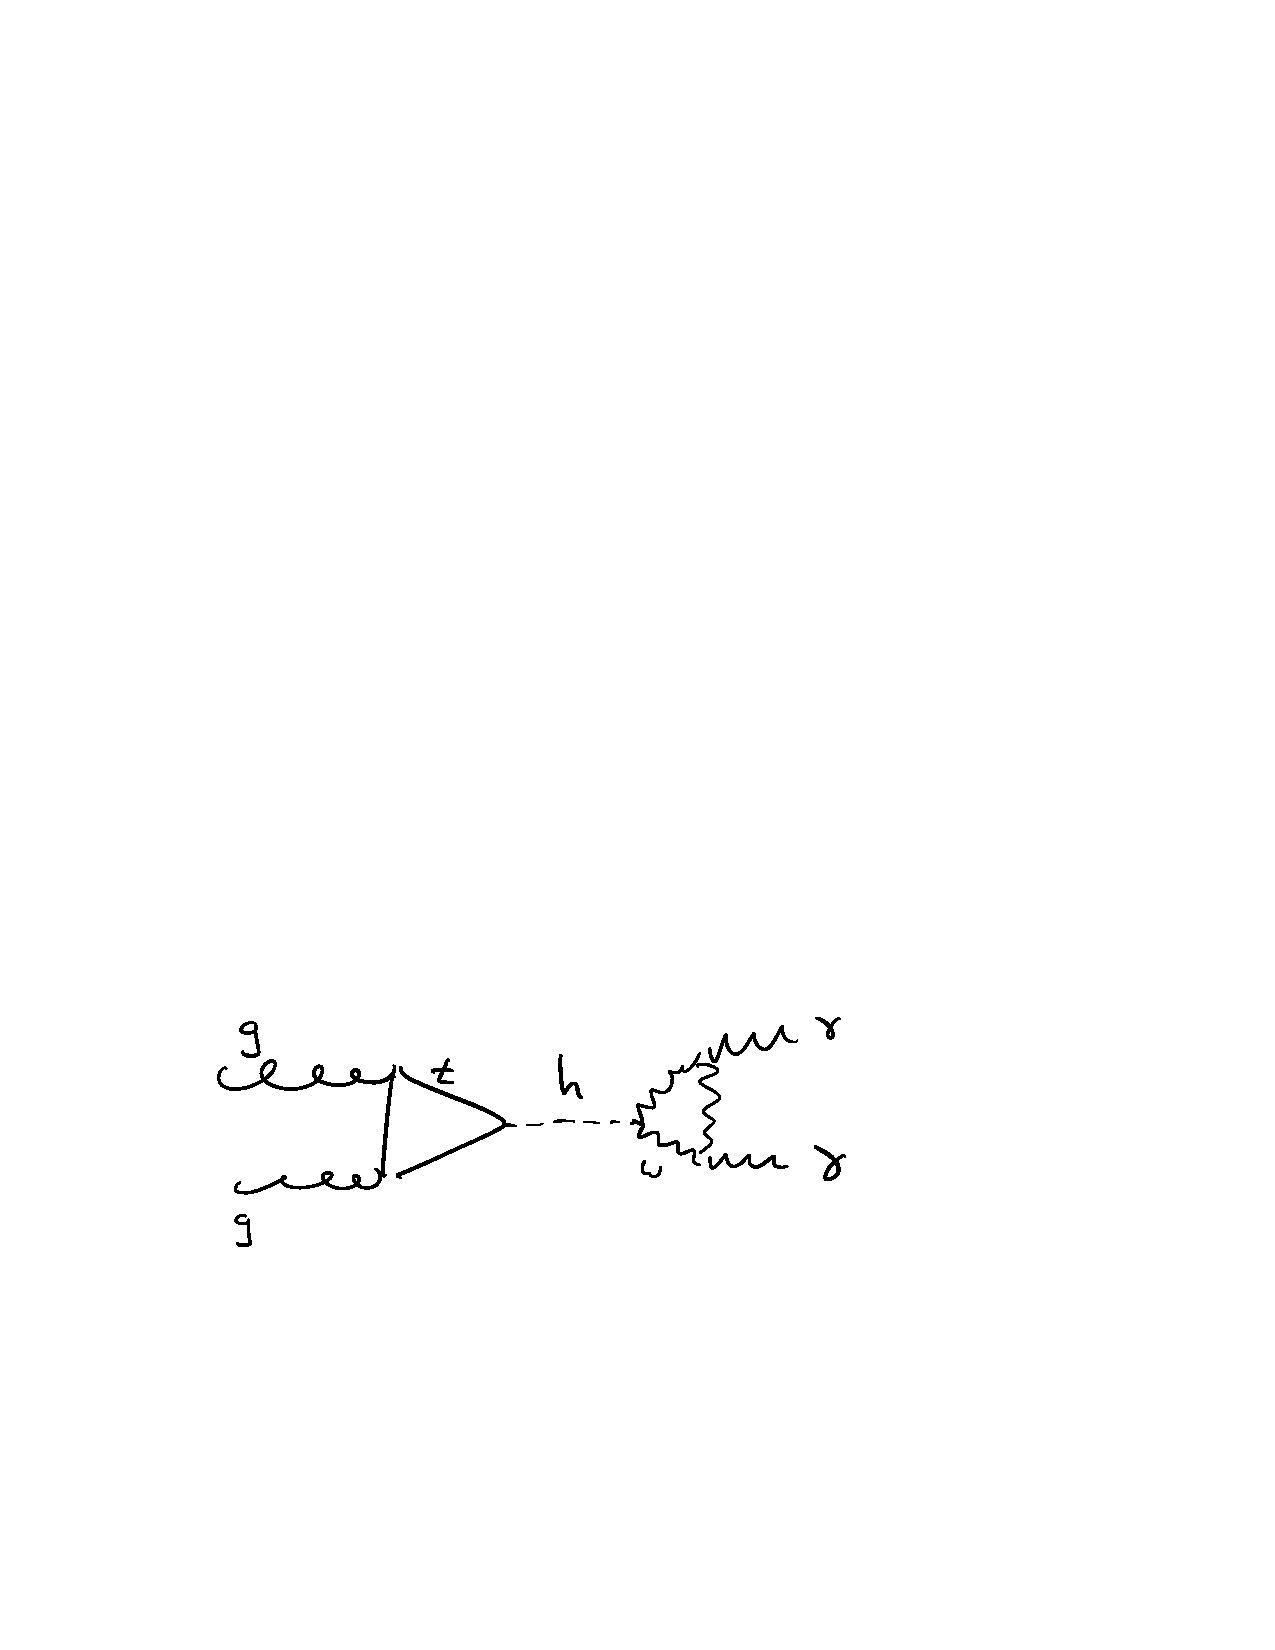
\includegraphics[width=0.3\textwidth]{./ggHgamgam.pdf}
%\ec
%
%\item[b)]{ Why is Higgs boson production so much rarer then W or Z production despite the fact that their masses are similar?   
%\bc
%Small couplings to stuff inside the proton (which is light), need 2nd order diagrams with large coupling to top, Ws and Z.
%\ec
% }
%\end{itemize}
%
%\vspace*{0.5in}

\clearpage

\textbf{11) Higgs-Lepton interactions } \hfill \textit{(4 points)}\\
The coupling of the Higgs field to leptons can be studied by looking for detector signals where the Higgs boson decays to pairs leptons.
Which of the possible decay modes would be the best way to do this.  Justify your answer.

\bc
Higgs to $\tau\tau$ as it has the largest mass and the Higgs coupling scales with mass. 
Will also give credit for Higgs to $\mu\mu$ if you comment that $\tau$ are hard to detector/measure
\ec

\vspace*{0.2in}

\textbf{12) Interaction Symmetries } \hfill \textit{(9 points)} \\ 
In the first part of the course we learned that the interactions of mass-less spin-1 particles must be described by group symmetries. 
\begin{itemize}
\item[a)]{How is the group symmetry of an underlying interaction related to the particle content ?

\bc
There is a gauge boson associated to each generator of the underlying symmetry.
\ec

}
\item[b)]{What are the symmetry groups of the electro-weak interaction in the SM ? 
\be
  SU(2)_L \times U(1)
\ee
}
\item[c)]{How does the observed physical particle content reflect this ? (Qualitatively, no formulas required.) 
\bc
The $W^\pm$ are two of the three generators of $SU(2)_L$.\\
The $Z$ and $\gamma$ are mixtures of the last $SU(2)_L$ generator and the U(1) generator
\ec
}

\end{itemize}

%\vspace*{0.5in}
%
%\textbf{14) Spontaneous Symmetry Breaking} \hfill \textit{(6 points)} \\ 
%\begin{itemize}
%\item[a)]{What is Spontaneous Symmetry Breaking  ? 
%
%\bc
%Case when the underlying potential or laws of physics respect a symmetry but the ground state of the system does not.
%\ec
%
% }
%\item[b)]{What properties of the fundamental particles is it responsible for describing ?
%\bc
%The masses of fundamental particles: the massive fermions and W and Z.
%\ec
%}
%\item[c)]{What experimental evidence do we have that spontaneous symmetry breaking is actually responsible for these properties?
%\bc
%Discovery of the Higgs boson.
%\ec
%}
%\end{itemize}



} % Begning Large
\end{document}
